Grupė - tai grupuojamo tinklo T subgrafas $G= \{V, E, u\}$. Subgrafo G šaltiniai $s_i$ yra:
\begin{enumerate}
	\item  tinklo šaltinis, jei jis yra subgrafo G viršūnių aibėje,
	\item  menamos viršūnės. Jei $\exists x: x \in V$ ir grupė $G_i : G_i \neq G$ turi viršūnę y, kuri nepriklauso grafui G, bei egzistuoja briauna $y \rightarrow x$, tai egzistuoja menama viršūnė x' ir briauna $x' \rightarrow x$, kurios pralaidumas yra lygus grupės $G_i$ maksimaliam srautui su tikslu x.
\end{enumerate}
subgrafo G tikslai $t_i$ yra:
\begin{enumerate}
	\item  tinklo tikslas, jei jis yra subgrafo G viršūnių aibėje,
	\item  menama viršūnė. Jei $\exists x: x \in V$ ir grupė $G_i : G_i \neq G$ turi viršūnę y, kuri nepriklauso grafui G, bei egzistuoja briauna $x \rightarrow y$, tai egzistuoja menama viršūnė x' ir briauna $x \rightarrow x'$, kurios pralaidumas yra lygus briaunos $x \rightarrow y$ pralaidumui.
\end{enumerate}

Kiekviena tinklo T viršūnė v priklauso tik vienai grupei. Kiekviena tinklo T briauna e priklauso tik vienai grupei, nebent $e = x \rightarrow y : x \in G_i, y \in G_j, i \neq j$

Pavyzdys: tarkime turime tinklą $G = {V={s, a, b, c, d, t}, E={s  \rightarrow a, a \rightarrow b, b \rightarrow c. c \rightarrow d, d \rightarrow t}}$, kuris yra sugrupuotas į grupes, kurių V yra lygūs {s, a}, {b, c}, {d, t}. Šis grupavimas pavaizduotas paveikslėlyje - \ref{fig:grupavimas}.
\begin{figure}[h]
	\caption{Grupavimo pavyzdys}
	\centering
	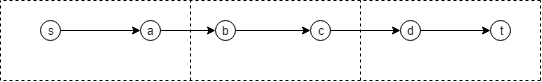
\includegraphics[width=\textwidth]{img/grupes_pavyzdziui.png}
	\label{fig:grupavimas}
\end{figure}

Tada subgrafo {b, c} šaltinis yra menama viršūnė $s_a$, kuri yra sujungta briauna, kurios pralaidumas yra subgrafo {s, a} maksimalus srautas iki tikslo b, o tikslas yra d.